
\documentclass[tikz,border=0pt]{standalone}
\usepackage{graphicx}
\usepackage{tikz}
\usetikzlibrary{shapes,shadows,calc}

\definecolor{cardback}{RGB}{10,10,25}
\definecolor{cardframe}{RGB}{150,100,200}
\definecolor{titletext}{RGB}{255,220,150}
\definecolor{bodytext}{RGB}{220,220,255}

\begin{document}
\begin{tikzpicture}

% Card background
\fill[cardback] (0,0) rectangle (8,11);

% Frame
\draw[cardframe, line width=2pt, rounded corners=5pt] (0.2,0.2) rectangle (7.8,10.8);
\draw[cardframe, line width=1pt, rounded corners=5pt] (0.4,0.4) rectangle (7.6,10.6);

% Title section
\fill[cardframe!30!cardback] (0.5,9.5) rectangle (7.5,10.5);
\node[titletext, font=\Large\bfseries] at (4,10) {G2E6};

% Archetype name
\node[titletext, font=\large\itshape] at (4,9.2) {The Hexagonal Cubic};

% Image section (centered square)
\node at (4,6) {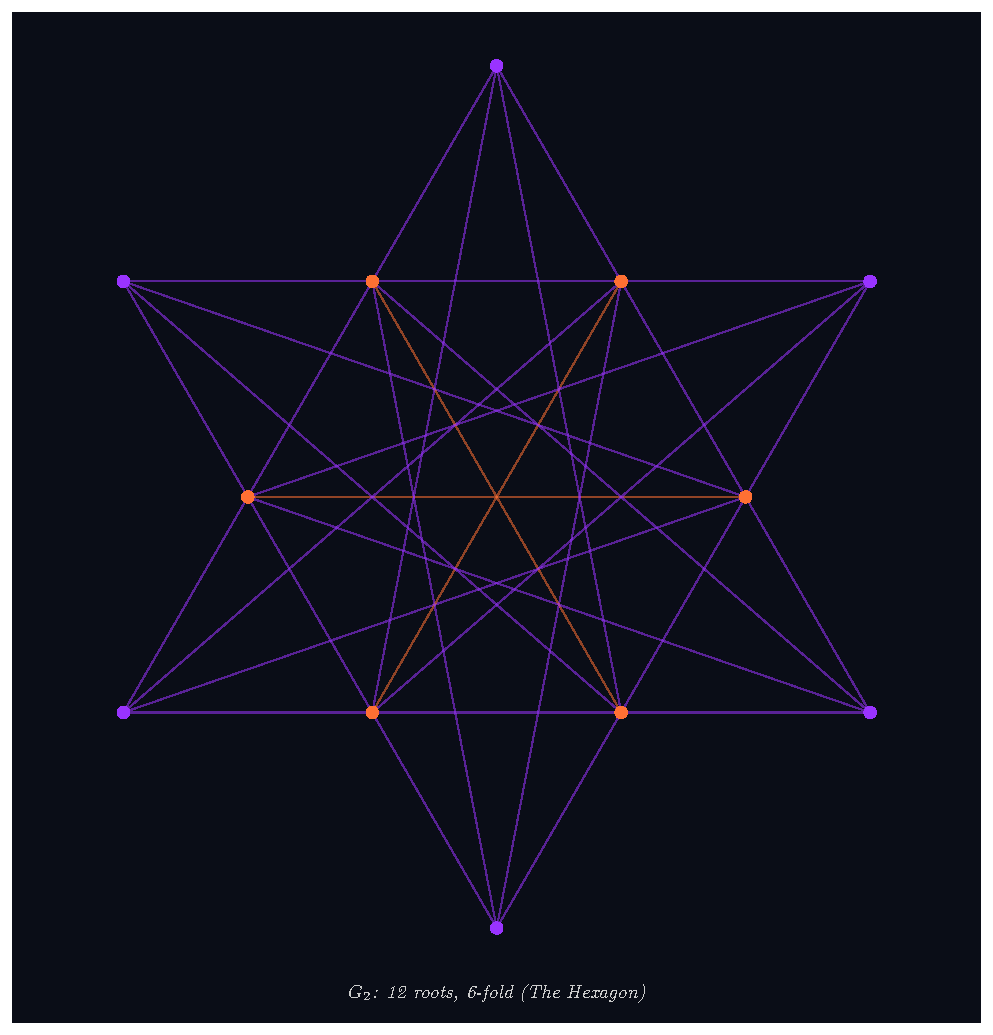
\includegraphics[width=6cm]{g2_roots.pdf}};

% Properties box
\fill[cardframe!20!cardback] (0.6,3.8) rectangle (7.4,4.8);
\node[bodytext, font=\small, align=left, text width=6.5cm] at (4,4.3) {
\textbf{Rank:} 8 \\
\textbf{Decomposition:} G2 $\times$ E6 \\ \textbf{Type:} Hexagon + Cubic \\ \textbf{Rank:} 2 + 6
};

% Quote section
\node[bodytext, font=\small\itshape, align=center, text width=6.5cm] at (4,2.5) {
``Six petals enfolding the trinity''
};

% Footer
\node[bodytext!50, font=\tiny] at (4,0.5) {Carter Class • W(E8) Conjugacy};

\end{tikzpicture}
\end{document}
